\documentclass{aa}
% \documentclass[referee]{aa}
\usepackage[varg]{txfonts}
\usepackage[separate-uncertainty=true,
            multi-part-units=single]{siunitx}
\usepackage[version=3]{mhchem}
\usepackage{amsmath}
\DeclareMathOperator{\sign}{sign}
\newcommand{\pluseq}{\mathrel{+}=}
\newcommand{\minuseq}{\mathrel{-}=}

\sisetup{range-units = single}
\sisetup{range-phrase = -}

\def\eps{\varepsilon}
\def\aap{A\&A}
\def\eprint{e-prints}
\def\apj{ApJ}
\def\apjs{ApJS}
\def\apjl{ApJL}
\def\mnras{MNRAS}
\def\aj{AJ}
\def\nat{Nature}
\def\aaps{A\&A Supp.}
\def\prd{Phys. Rev. D}
\def\prl{Phys. Rev. Lett.}
\def\araa{ARA\&A}

\begin{document}


\title{SWEET-Cat update and MOOGme}
\subtitle{A new minimization procedure for high quality spectra}


\author{ D.~T.~Andreasen\inst{1,2}
    \and S.~G.~Sousa\inst{1}
    \and N.~C.~Santos\inst{1,2}
    \and M.~Tsantaki\inst{3}
    \and G.~Teixeira\inst{1}
    \and L.~Su\'arez-Andr\'es\inst{4,5}
    \and A.~Mortier\inst{6}
}


\institute{
Instituto de Astrof\'isica e Ci\^encias do Espa\c{c}o, Universidade do Porto, CAUP, Rua das Estrelas, 4150-762 Porto, Portugal
\email{daniel.andreasen@astro.up.pt}
\and
Departamento de F\'isica e Astronomia, Faculdade de Ci\^encias, Universidade do Porto, Rua Campo Alegre, 4169-007 Porto, Portugal
\and
Instituto de Radioastronom\'ia y Astrof\'isica, IRyA, UNAM, Campus Morelia, A.P. 3-72, 58089 Michoac\'an, Mexico
\and
Instituto de Astrof\'isica de Canarias, E-38205 La Laguna, Tenerife, Spain
\and
Depto. Astrof\'isica, Universidad de La Laguna (ULL), E-38206 La Laguna, Tenerife, Spain
\and
SUPA, School of Physics and Astronomy, University of St Andrews, St Andrews KY16 9SS, UK
}





\date{Received ...; accepted ...}

\abstract
% Context
{}
% Aims
{}
% Methods
{}
% Results
{}
% Conclusions
{}



\keywords{data reduction: high resolution spectra --
          stars individual: Arcturus --
          stars individual: HD010853}
\maketitle



\section{Introduction}
\label{sec:introduction}
The study of extrasolar planetary systems is an established field of research.
To date, nearly 3500 extrasolar planets have been discovered around almost 2500
solar-type stars\footnote{For an updated table we refer to
\url{http://www.exoplanet.eu}}. Most of these have been found thanks to the
incredible precision achieved in photometric transit and radial velocity
methods. The increasing number of exoplanets allows us to do statistical studies
of the newfound worlds by analyzing their internal structure, atmospheric
composition, and planetary composition.

Precise and accurate planetary parameters (mass, radius, and mean density) are
needed to distinguish between solid rocky, water rich, gaseous, or otherwise
composed planets. A key aspect to this progress is the characterization of the
planet host stars. For instance, precise and accurate stellar radii are critical
if we want to measure precise and accurate values of the radius of a transiting
planet \citep[see e.g.][]{Torres2012,Mortier2013}. The determination of the
stellar radius is in turn dependent on the quality of the derived stellar
atmospheric parameters such as the effective temperature.

We continue the work of \citet{Santos13} by deriving atmospheric parameters,
namely the effective temperature ($T_\mathrm{eff}$), surface gravity ($\log g$),
metallicity ([Fe/H], where iron often is used as a proxy for the total
metallicity), and the micro turbulence ($\xi_\mathrm{micro}$) in a homogeneous
way for a sample of planet host stars. This, in turn, allows us to study new
correlations between planets and their hosts in a homogeneous way,  or gain
higher statistical certainty on the already discovered correlations.

The analysis of high quality spectra, i.e. spectra with high spectral resolution
and an high  signal to noise ratio (SNR), serves an important role in the
derivation of stellar atmospheric parameters. Nevertheless, spectral analysis is
a time consuming method. There has been an increase of the amount of  optical
high-resolution spectrographs available and, additionally, a number of near-IR
spectrographs are either planned or are already available making the task of
analyzing the increasing amount of spectra even more crucial.

In the era of large data sets, computation time has to be decreased as much as
possible without compromising the quality of the results. In the light of this
we have developed a tool to derive atmospheric parameters in a fast and robust
way using standard spectroscopic methods. This works well for optical spectra
which we demonstrate in Section~\ref{sub:Testing_MOOGme} using the line list
from \citet{Sousa2011}. This tool also ships with a line list for near-IR
spectra using the line list presented recently in \citet{Andreasen2016}. The
tool is provided to the community as an easy to use web tool to avoid any
problems with installations. The tool is described in detail in
Section~\ref{sec:MOOGme}.



\section{Data}
\label{sec:data}
We obtain 43 spectra related to this work by using the UVES \citep{UVES}, FEROS
\citep{FEROS}, and FIES \citep{FIES} spectrographs. The rest (18) spectra were
found in various archives. Additionally, we use spectra from HARPS \citep{HARPS}
and ESPaDOnS \citep{ESPADONS}. Some characteristics of the spectrographs are
presented in Table~\ref{tab:instruments} with the mean SNR for the spectra used.
The SNR for each star can be seen in Table~\ref{tab:results} along with the
atmospheric parameters of the stars.

We obtain the spectra with the highest possible resolution for a given
spectrograph, and in cases with multiple observations, we include all unless a
spectrum is close to the saturation limit for a given spectrograph. For multiple
spectra, we combine them after first correcting the radial velocity (RV) and
using a sigma clipper to remove cosmic rays. The individual spectra are then
combined to a single spectrum for a given star to increase the SNR. This single
spectrum is used in the analysis below. For most of the spectra in the archive
included here, several spectra were combined as described above, while for the
observations dedicated to this work, the spectrum would be a single spectrum.
This is mostly due to the difference in science cases behind the observations.
E.g. the HARPS spectra were used for RV monitoring or follow up of the
exoplanet(s).

\begin{table}[htb!]
    \caption{Spectrographs used for this paper with their spectral resolution,
             wavelength coverage, and typical (mean) SNR from the spectra used.}
    \label{tab:instruments}
    \centering
    \begin{tabular}{llll}
      \hline\hline
      Spectrograph & Resolution & spectral coverage           &   Mean SNR  \\
      \hline
      UVES         &    110 000 & $\SIrange{420}{1100}{nm}$   &   212       \\
      FEROS        &     48 000 & $\SIrange{350}{920}{nm}$    &   208       \\
      HARPS        &    115 000 & $\SIrange{378}{691}{nm}$    &   642       \\
      FIES         &     67 000 & $\SIrange{370}{730}{nm}$    &   763       \\
      ESPaDOnS     &     81 000 & $\SIrange{370}{1050}{nm}$   &   775       \\
      \hline
    \end{tabular}
\end{table}




\section{MOOGme}
\label{sec:MOOGme}
MOOGme (acronym for MOOG made easy) is a web
tool\footnote{\url{super-cool-address-with-MOOGme}} for analyzing spectra.
MOOGme is written in Python and works as a wrapper around MOOG
\citep[][version 2014]{Sneden1973}, and ARES \citep{Sousa2015a} for an all-in-one
tool. MOOG is a radiative transfer code under the assumption of local
thermodynamic equilibrium (LTE). ARES is a tool to automatically measure
equivalent widths (EW) from a spectrum given a line list. MOOGme has three
different modes: i) Measure EWs using ARES, ii) derive stellar parameters from a
set of measured \ion{Fe}{I} and \ion{Fe}{II} line EWs, and iii) abundances
derivation for 15 elements, all described below. The model atmospheres are
formatted in a grid of Kurucz Atlas 9 plane-parallel, 1D static model
atmospheres \citet{Kurucz1993}. MOOGme can also manage the new grid of Atlas
models calculated by \citet{Meszaros2012} for the APOGEE survey and the MARCS
models \citep{Gustafson2008}. The interpolation from the grid is calculated from
a geometric mean for effective temperature, surface gravity and metallicity.



\subsection{EW measurements}
\label{sub:EW_measurements}
The EWs are strongly correlated with the atmospheric parameters. Measurements of
the EW can be done manually using a tool like IRAF, but often when dealing with
a large sample of stars this is not a suitable way to deal with the task.
Therefore tools like ARES exist which can measure the EWs of spectral lines
automatically. To use this mode of MOOGme, it just needs a spectrum (format
should be 1D fits for ARES to read it) and a line list. For the latter, MOOGme
is shipped with some line lists ready to use, in the format suitable for MOOGme.
The output will be a line list in the format required for MOOG. The output can
be used for either the EW method or the abundance method, both described below.

The line lists shipped with MOOGme are presented in Table~\ref{tab:linelists}.
These line lists are all calibrated for the Sun, i.e. the oscillator strengths
for each absorption line are changed so the line with the measured EW from a
solar spectrum return solar abundance for the given element.

\begin{table}[htb!]
    \caption{The line lists provided with MOOGme. The first two line lists
             are for parameter determination while the last line list is
             used to derive abundances for 15 different elements.}
    \label{tab:linelist}
    \centering
    \begin{tabular}{lrrl}
      \hline\hline
      Line list             & \ion{Fe}{I}/\ion{Fe}{II} & Elements   & Usage      \\
      \hline
      \citet{Sousa2008a}    &  263/36                  &  1         & Parameters \\
      \citet{Tsantaki2013}  &  120/17                  &  1         & Parameters \\
      \citet{Andreasen2016} &                          &  1         & Parameters \\
      \citet{Neves2009}     &  -/-                     & 15         & Abundances \\
      \hline
    \end{tabular}
\end{table}



\subsection{EW method}
\label{sub:EW_method}
The standard determination of spectroscopic parameters for solar-type stars
starts by measuring the EW of selected and well-defined absorption lines. Then
we translate these measurements into individual line abundances, assuming a
given atmospheric model. We obtain the correct stellar parameters by imposing
excitation and ionization balance for the iron species.

\begin{itemize}
    \item The effective temperature has a strong influence on the correlation
          of iron abundance with the excitation potential (excitation balance).
          We obtain the $T_\mathrm{eff}$ when \ion{Fe}{I} abundance shows no
          dependence on the excitation potential, i.e., the slope of abundance
          versus excitation potential is zero.
    \item Surface gravity is derived from the ionization balance of \ion{Fe}{I}
          and \ion{Fe}{II} abundances. Therefore, the abundance of neutral iron
          should be equal to the abundance of ionized and consistent with the
          one of the input model atmosphere.
    \item Microturbulence is connected with the saturation of the stronger iron
          lines. However, the abundances for weak and strong lines of a certain
          species (in our case iron) should be the same independent of the value
          of $\xi_\mathrm{micro}$. Iron abundances should show no dependence on
          the reduced equivalent width, i.e. the slope of abundance vs the
          reduced EW is zero.
\end{itemize}


With measured EWs of \ion{Fe}{I} and \ion{Fe}{II} lines we calculate abundances
using a stellar atmosphere model for a given set of atmospheric parameters
($T_\mathrm{eff}$, $\log g$, [Fe/H], and $\xi_\mathrm{micro}$). By removing
correlations between the measured abundances (through the measured EWs) and the
excitation potential (EP) and reduced EW ($\log(EW/\lambda)$) we can constrain
$T_\mathrm{eff}$ and $\xi_\mathrm{micro}$. By obtaining ionization balance
between \ion{Fe}{I} and \ion{Fe}{II} (that is the average abundance of all
\ion{Fe}{I} lines are equal to the average abundance of all \ion{Fe}{II} lines)
we constrain $\log g$. Lastly, we change the input [\ion{Fe}/\ion{H}] to match
that of the average output [\ion{Fe}/\ion{H}]. Hence we have four criteria to
minimize simultaneously:

\begin{enumerate}
    \item The slope between abundance and excitation potential ($a_\mathrm{EP}\le0.001$).
    \item The slope between abundance and reduced EW ($a_\mathrm{RW}\le0.003$).
          We use 0.003 rather than 0.001 since this slope varies more rapidly
          with small changes in atmospheric parameters.
    \item The difference between the average abundances of \ion{Fe}{I} and
          \ion{Fe}{II} ($\Delta\ion{Fe}{}\le0.01$).
    \item Input and output metallicity should be equal.
\end{enumerate}
These criteria we denote as indicators for the physical parameters which we are
trying to minimize for. We denote this method for obtaining stellar parameters
for the EW method.

\begin{figure}[tpb]
    \centering
    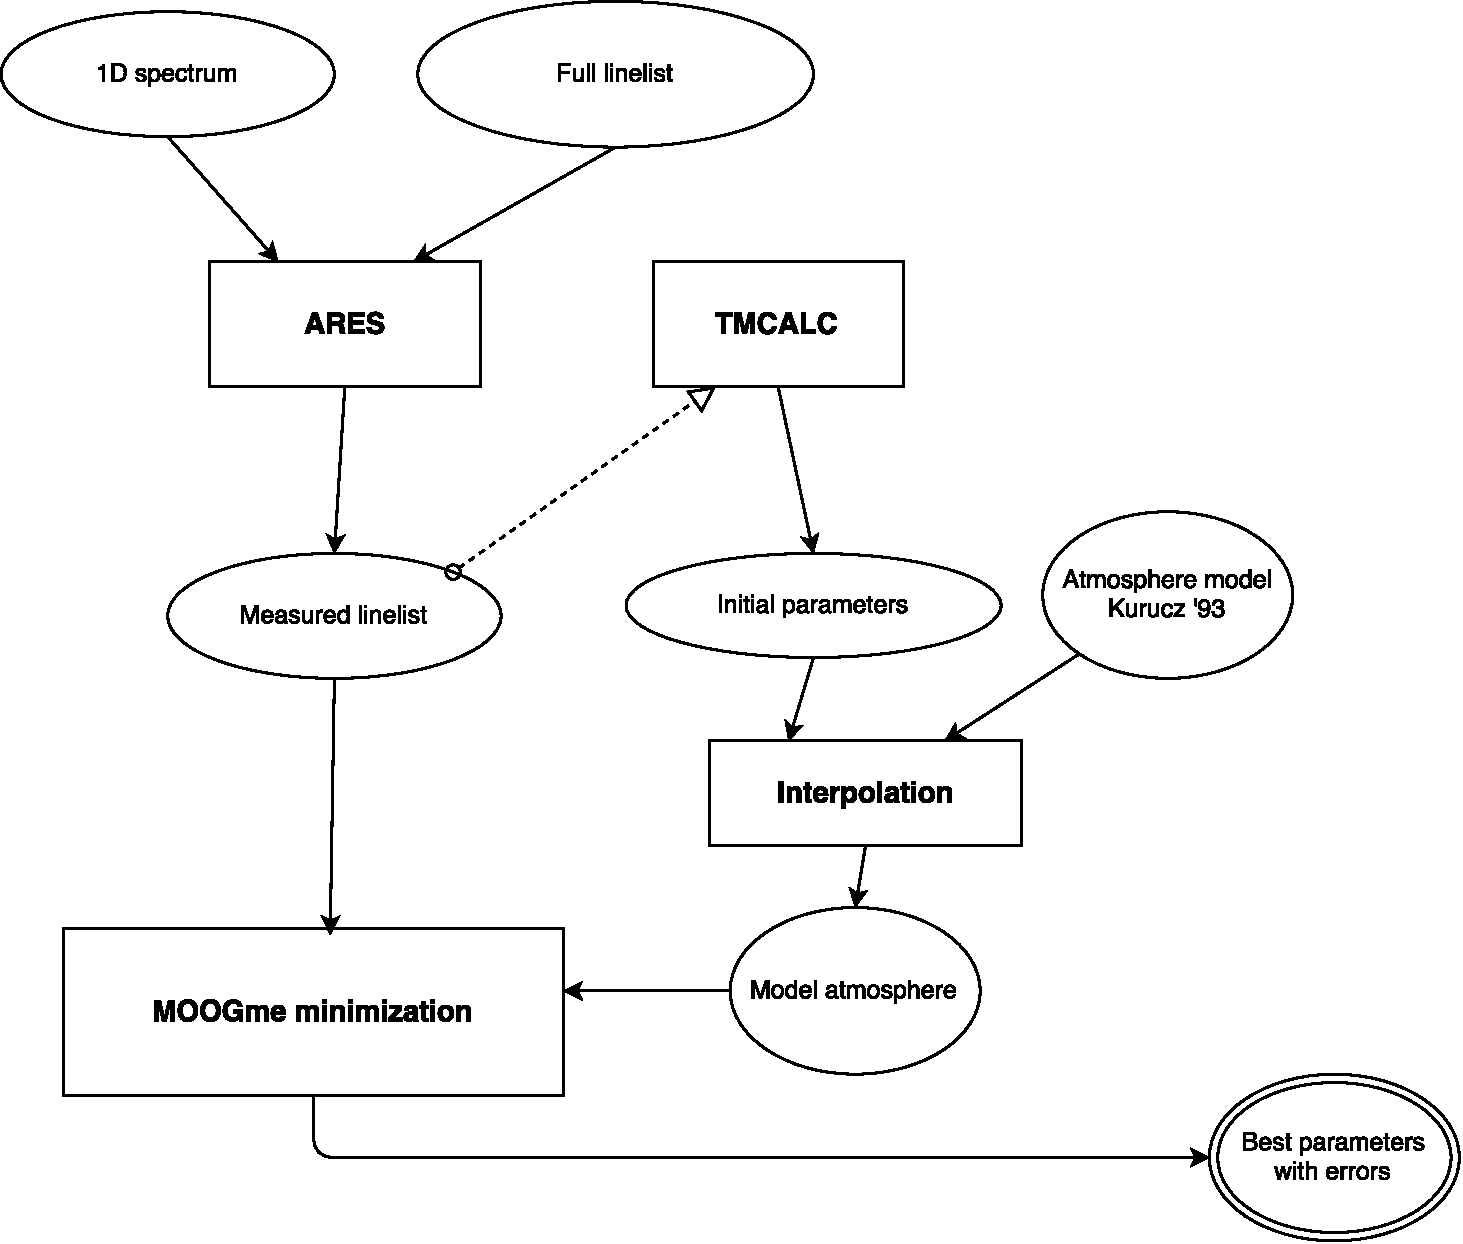
\includegraphics[width=1.0\linewidth]{figures/MOOGme_general.pdf}
    \caption{A general overview over MOOGme from spectrum to parameters.}
    \label{fig:MOOGme_general}
\end{figure}

There exists many minimization routines available in Python. Most commonly known
are the ones from the SciPy ecosystem\footnote{\url{http://scipy.org}}. There
are some pros and cons with using proprietary minimization routines. Pros are
that it is already written, and usually there is good documentation for
libraries such as SciPy. Cons in this situation is, that most minimization
routines do not work well with vector functions returning another vector:
\begin{align}
    f(\{T_\mathrm{eff}, \log g, [Fe/H], \xi_\mathrm{micro}\}) = \{a_\mathrm{EP}, a_\mathrm{RW}, \Delta\ion{Fe}, \ion{Fe}{I}\}.
\end{align}
A work around is to combine the criteria into one single criteria by e.g. adding
them quadratically and minimize that expression instead. Thus we have a vector
function returning a scalar:
\begin{align}
    f(\{T_\mathrm{eff}, \log g, [Fe/H], \xi_\mathrm{micro}\}) &= \sqrt{a_\mathrm{EP}^2 + a_\mathrm{RW}^2 + \Delta\ion{Fe}{}^2}.
\end{align}
The minimization routines are also not physical in the sense that they are not
optimized for the problem. These two cons were incitement for writing a
minimization routine optimized for the problem at hand. Here is how it works.

\begin{enumerate}
    \item Run MOOG once with a user defined initial parameters (default is
          solar) and calculate $a_\mathrm{EP}$, $a_\mathrm{RW}$, and
          $\Delta$\ion{Fe}.
    \item Change the atmospheric parameters ($T_\mathrm{eff}$, $\log g$,
          [\ion{Fe}/\ion{H}], $\xi_\mathrm{micro}$) according to the size of the
          indicator. A parameter is only changed if it is not fixed.
    \begin{itemize}
        \item $a_\mathrm{EP}$: Indicator for $T_\mathrm{eff}$. If this value
              is positive, then increase $T_\mathrm{eff}$.
        \item $a_\mathrm{RW}$: Same as above but for $\xi_\mathrm{micro}$.
        \item $\Delta$\ion{Fe}{}: Positive $\Delta$\ion{Fe}{} means $\log g$
              should be decreased and vice versa.
        \item For [\ion{Fe}/\ion{H}] it is changed to the output [\ion{Fe}/\ion{H}]
              in each iteration.
    \end{itemize}
    \item If the new parameters have already been used in a previous iteration,
          then change them slightly. This is done by drawing a random number from
          a Gaussian distribution with a mean at the current value and a sigma
          equal to the absolute value of the indicator.
    \item Calculate a new atmospheric model by interpolating a grid so we have
          the requested parameters and run MOOG once again.
    \item For each iteration save the parameters used and the quadratic sum of
          the indicators. If we do not reach convergence, then return the best
          found parameters.
\end{enumerate}
This whole process is schematically shown in Figure~\ref{fig:MOOGme_general} and
the minimization routine itself in Figure~\ref{fig:MOOGme_minimization}. The
stepping follows these simple equations:
\begin{align}
    T_\mathrm{eff}     &\pluseq \SI{2000}{K} a_\mathrm{EP}   \\
    \xi_\mathrm{micro} &\pluseq \SI{1.5}{km/s} a_\mathrm{RW} \\
    \log g             &\minuseq \Delta\ion{Fe}.
\end{align}
The metallicity is corrected at each step so the input metallicity matches that
of the output metallicity of the previous iteration. The functional form for
changing the parameters were found by changing one parameter, e.g.
$T_\mathrm{eff}$, while keeping the other parameters fixed at their convergence
values. A linear fit was applied to $T_\mathrm{eff} - T_\mathrm{eff,0}$ vs.
$a_\mathrm{EP}$ in order to get the slope. Since we ignore all interdependencies
between the parameters in doing so, we lower the slopes above a little and
arrive to these very simple equations.

The error estimates is based on the same method presented in
\citet{Gonzalez2000}, which is also described in details in
\citet{Santos2003,Andreasen2016}.

\begin{figure}[tpb]
    \centering
    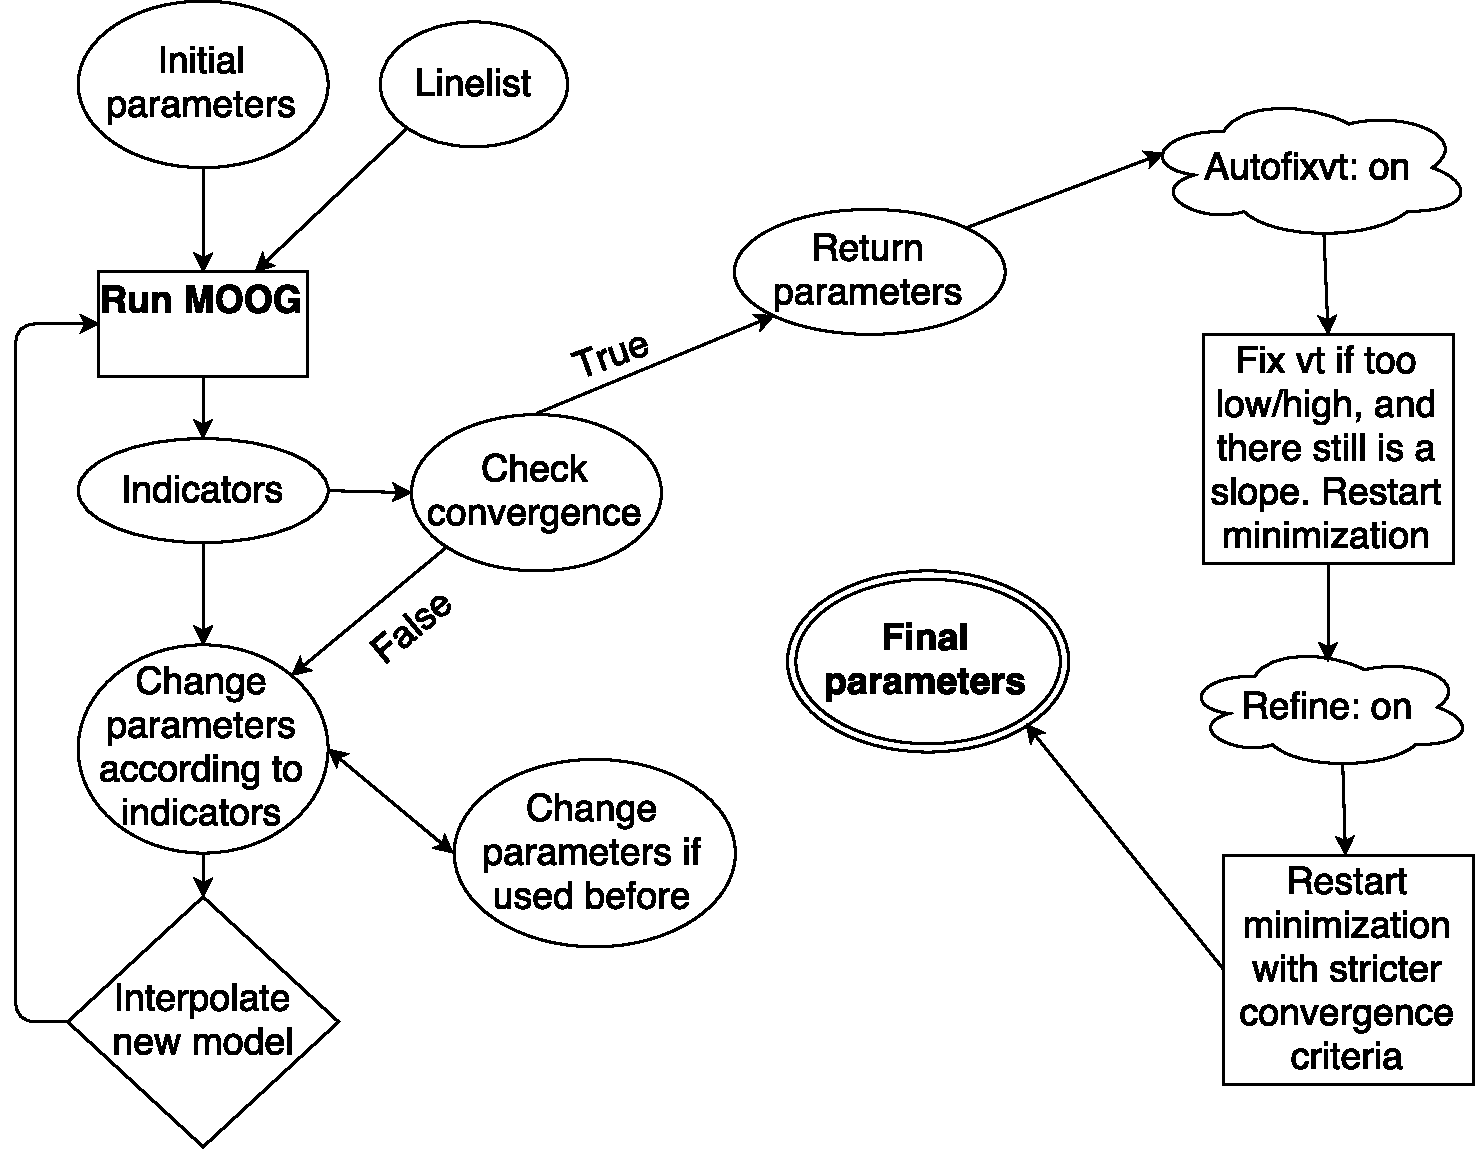
\includegraphics[width=1.0\linewidth]{figures/MOOGme_minimization.pdf}
    \caption{A schematic overview over the minimization for MOOGme with the
    EW method.}
    \label{fig:MOOGme_minimization}
\end{figure}

By using the indicators like this, we can relative fast reach convergence.
Typical calculation time for an FGK dwarf with a high quality spectrum is around
$\SI{2}{min}$.

\subsubsection{Options}
\label{subs:EWoptions}
It is possible to run the EW method with a set of different options which
will be described here.

\begin{itemize}
    \item \emph{fixteff}: Fix $T_\mathrm{eff}$ and derive the other parameters.
          Same is available for $\log g$ (\emph{fixlogg}), [\ion{Fe}/\ion{H}]
          (\emph{fixfeh}), and $\xi_\mathrm{micro}$ (\emph{fixvt}). One or more parameters
          can be fixed. When one or more parameters are fixed, the corresponding
          indicator will be ignored for each iteration, thus the parameter itself
          will not be changed.
    \item \emph{outlier}: Remove outliers after the first run with the minimization
          routine and restarting the minimization from the previous best
          parameters. The options are to remove all outliers above $3\sigma$
          once or iteratively, or remove one outlier above $3\sigma$ once or
          iteratively.
    \item \emph{autofixvt}: If the minimization routine does not converge and
          $\xi_\mathrm{micro}$ is close to 0 or 10 with a significant
          $a_\mathrm{RW}$ (numerically bigger than 0.05), then fix
          $\xi_\mathrm{micro}$. This option was added since we saw this behaviour
          in some cases. The solution was typically to restart the minimization
          manually with $\xi_\mathrm{micro}$ fixed.
    \item \emph{refine}: After the minimization is done, run it again from the best
          found parameters but with more strict criteria. If this option is set,
          it will always be the last step (after removal of outliers). The
          convergence criteria can be changed by the user, but we recommend
          using the defaults provided above.
    \item \emph{tmcalc}: Use TMCalc \citep{Sousa2012} to fast estimate the
          $T_\mathrm{eff}$ and $[\ion{Fe}/\ion{H}]$ using the raw output from
          ARES. We then assume solar surface gravity ($\SI{4.44}{dex}$) and
          estimate $\xi_\mathrm{micro}$ based on an empirical relation (see below).
\end{itemize}
If $\xi_\mathrm{micro}$ is fixed it is changed at each iteration according to an
empirical relation. For dwarfs it follows the one presented in
\citet{Tsantaki2013} and for giants it follows the one presented in
\citet{Adibekyan2015}.

We use the line list presented in \citet{Sousa2008a}. However, this line list
does not work well for cool stars. This was fixed in \citet{Tsantaki2013} by
removing some lines from \citet{Sousa2008a}. For stars cooler than \SI{5200}{K}
we automatically rederive the atmospheric parameters after removing lines so the
line list resemble that of \citet{Tsantaki2013}.

All restarts of the minimization routine is done with initial condition at the
last found best parameters.


\subsection{Abundance method}
\label{sub:Abundance_method}

With the line list from \citet{Neves2009} with 15 different elements it is
possible to measure abundances for these elements by combining the ARES mode to
measure the EWs and the EW method mode to obtain the atmospheric parameters. The
abundances are saved to a table.


\subsection{Testing MOOGme}
\label{sub:Testing_MOOGme}
To test the EW method implemented in MOOGme we derive parameters from the 582
sample by \citet{Sousa2011}. We use ARES2 to measure the EWs. ARES can give an
estimate on the signal to noise ratio (SNR) by analyzing the continuum in given
intervals. For solar type stars the following intervals are working well:
\SIrange{5764}{5766}{\angstrom}, \SIrange{6047}{6053}{\angstrom}, and
\SIrange{6068}{6076}{\angstrom}. From the estimated SNR, ARES can give an
estimate on the very important \emph{rejt} parameters \citep[see][for more
information]{Sousa2015a}. After measuring the EWs with ARES, we use the MOOGme
minimization described in Section~\ref{sub:EW_method} to determine the stellar
atmospheric parameters. The results are presented in Figure~\ref{fig:MOOGmeTest}
which shows $T_\mathrm{eff}$, $\log g$, [\ion{Fe}/\ion{H}], and
$\xi_\mathrm{micro}$ for MOOGme against those of \citet{Sousa2011}.

\begin{figure*}[tpb]
    \centering
    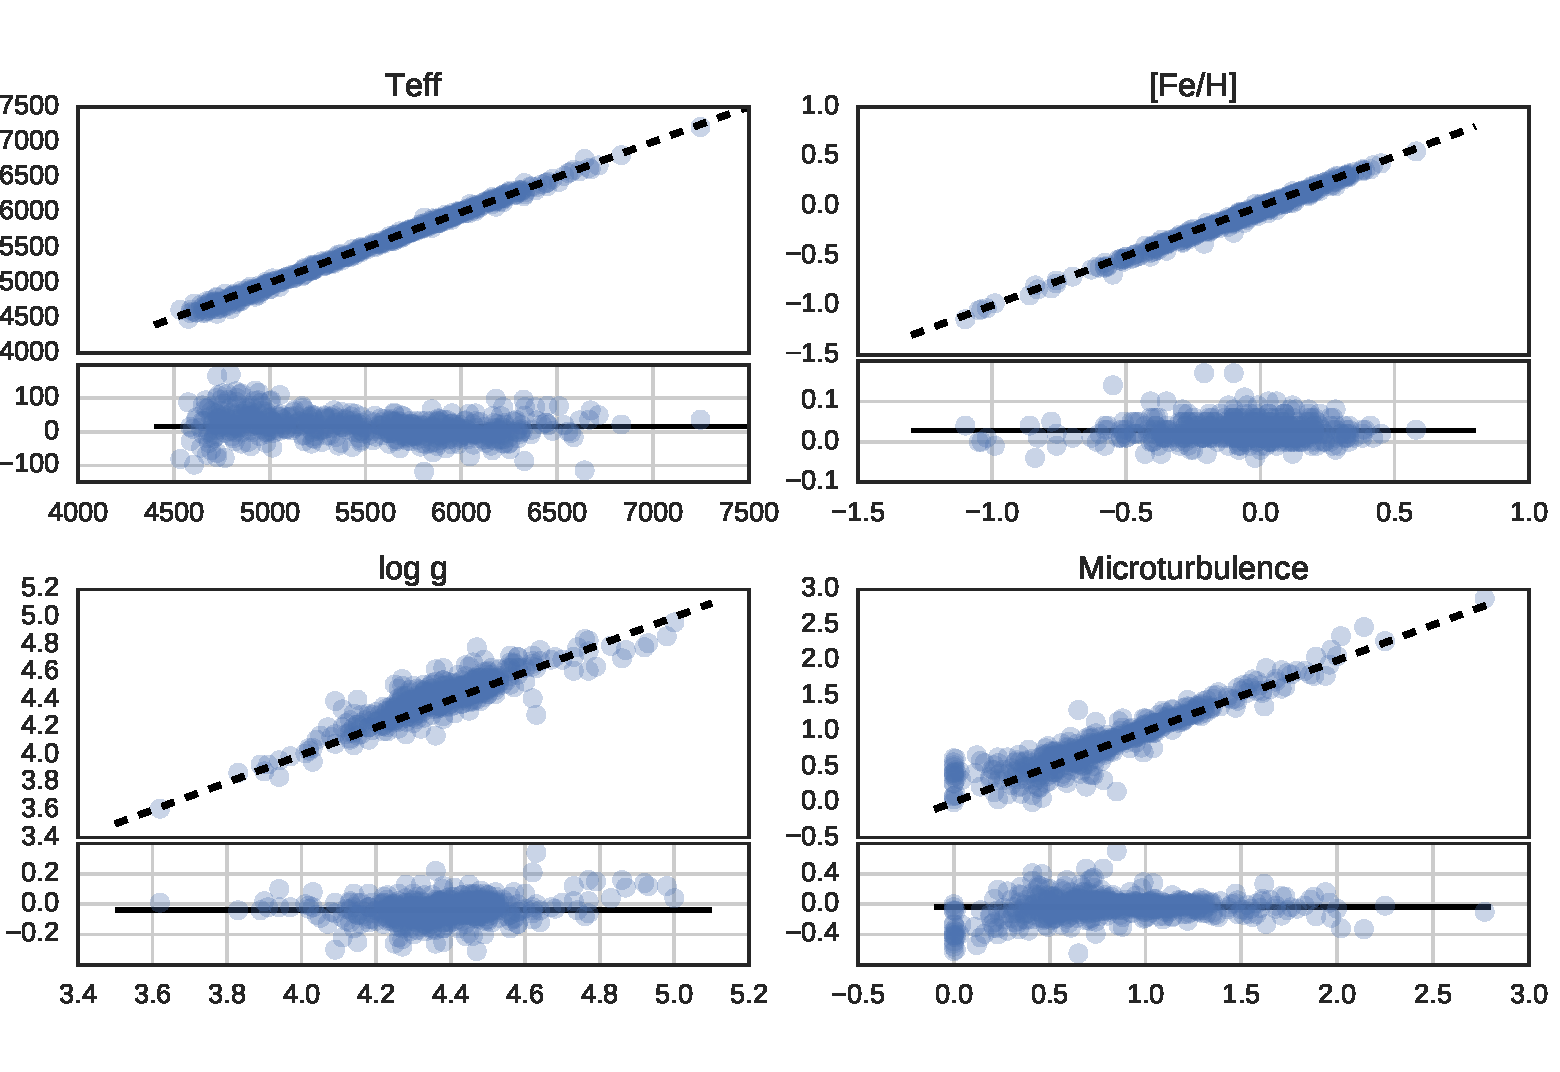
\includegraphics[width=1.0\linewidth]{figures/MOOGmeTest.pdf}
    \caption{Stellar atmospheric parameters derived by MOOGme compared
    to the sample by \citet{Sousa2011}.}
    \label{fig:MOOGmeTest}
\end{figure*}

The sample contains stars with $T_\mathrm{eff}$ too cold for the line list used.
As described in Section~\ref{sub:EW_method} we should then convert the line list
by \citet{Sousa2008a} to the line list presented in \citet{Tsantaki2013}.
However, since this line list was not available when \citet{Sousa2011} derived
parameters, we do not make this change in order to make a better test for
MOOGme.

The mean of the difference between parameters from \citet{Sousa2011} and those
by MOOGme are presented in Table~\ref{tab:MOOGmeTest}.

\begin{table}[htb!]
    \caption{The difference in derived parameters by \citet{Sousa2011}
    and MOOGme. Second column is the mean difference with EWs measured by
    ARES in MOOGme, while the third column is the mean difference using
    20 randomly stars with the exact same line list.}
    \label{tab:MOOGmeTest}
    \centering
    \begin{tabular}{lrr}
      \hline\hline
      Parameter             &  Mean difference         & Same line list        \\
      \hline
      $T_\mathrm{eff}$      &  $\SI{16(36)}{K}$        & $\SI{21(11)}{K}$      \\
      $\log g$              &  $\num{-0.04(7)}$        & $\num{-0.007(9)}$     \\
      $[\ion{Fe}/\ion{H}]$  &  $\num{0.03(2)}$         & $\num{0.004(9)}$      \\
      $\xi_\mathrm{micro}$  &  $\SI{-0.04(14)}{km/s}$  & $\SI{0.04(2)}{km/s}$  \\
      \hline
    \end{tabular}
\end{table}

We see small offsets that can be due to different versions of MOOG, measured
line lists, interpolation of atmosphere grid, and minimization routine. Most
likely the difference will be due to different used \emph{rejt} parameters in
ARES, which can alter the EWs and hence the parameters. We therefore randomly
selected 20 stars with different $T_\mathrm{eff}$ and used the line lists
directly from \citet{Sousa2011} to derive parameters. The results are presented
in the last column of Table~\ref{tab:MOOGmeTest}. We note that the $\log gf$
values from the original line lists by \citet{Sousa2011}, which used the MOOG
2002 version, were not changed for the 2014 version of MOOG. This might lead to
some errors as well. However, the offsets are very small and compatible with the
errors on parameters normally obtained from high quality spectra.


\subsection{Web interface}
\label{sub:Web interface}
NOTE: More will be written once we have a web page.

We provide a web interface for MOOGme. In the web interface it is possible to
use some of the line list provided with MOOGme to measure EWs of a spectrum (has
to be provided by the user). This can be used for all the available MOOGme
methods described above.

The web interface can be found at the following link
\url{super-cool-address-with-MOOGme}.



\section{New spectroscopic parameters for 61 planet hosts}
\label{sec:results}
Here we present the sample of 61 stars. We were unable to derive parameters for
HD77065. This is a spectroscopic binary according to \cite{Pourbaix2004}, and
the spectrum is contaminated with the companion star. This make EW measurement
very difficult, hence we exclude it from the sample.

Moreover we were not able to successfully derive parameters with this method
for Aldebaran, a well known red giant star. Even though the quality of the
spectra for a bright star like Aldebaran are available, the spectral type
is intrinsic difficult due to the low $T_\mathrm{eff}$ which can give arise to
molecular absorption in the optical. We also expect to see non-LTE effects for
this kind of spectral type. That we are not able to derive parameters for
Aldebaran is not a big concern, since it is well studied with other techniques,
and we can trust the parameters already listed in SWEET-Cat.

The remaining 61 stars are presented in Table~\ref{tab:results}.

\begin{table*}[htb!]
    \caption{The derived parameters for the 61 stars in our sample. The SNR
             is measured by ARES.}
    \label{tab:results}
    \centering
    \begin{tabular}{llllllll}
      \hline\hline
      % Add alternative name and SNR
      Star      & $T_\mathrm{eff}$ (K) &  $\log g$ (dex)     &  [Fe/H] (dex)        &  $\xi_\mathrm{micro}$ (km/s)   & $\xi_\mathrm{micro}$ fixed? & Instrument   & SNR   \\  %Program ID \\
      \hline
      WASP-37     &  $6024 \pm  58$      &  $4.70 \pm 0.06$	   &  $-0.15 \pm 0.05$    &  $1.34 \pm 0.09$             &             no              & FIES         &  250  \\
      WASP-44     &  $5612 \pm  80$      &  $4.47 \pm 0.30$    &  $ 0.17 \pm 0.06$    &  $1.32 \pm 0.13$             &             no              & UVES         &  125  \\  % 092.C-0695                                                                                                              \\
      WASP-52     &  $5197 \pm  83$      &  $4.47 \pm 0.30$    &  $ 0.15 \pm 0.05$    &  $1.16 \pm 0.14$             &             no              & UVES         &  125  \\  % 093.C-0219                                                                                                              \\
      WASP-58     &  $6103 \pm  64$      &  $4.68 \pm 0.08$	   &  $-0.10 \pm 0.04$    &  $1.36 \pm 0.11$             &             no              & FIES         &  293  \\
      WASP-60     &  $6330 \pm  64$      &  $4.66 \pm 0.09$	   &  $ 0.36 \pm 0.04$    &  $1.61 \pm 0.09$             &             no              & FIES         &  315  \\
      WASP-61     &  $6265 \pm 168$      &  $4.21 \pm 0.21$    &  $-0.38 \pm 0.11$    &  $1.44 \pm 0.02$             &             yes             & UVES         &  163  \\  % 094.C-0367                                                                                                              \\
      WASP-72     &  $6570 \pm  85$      &  $4.71 \pm 0.13$    &  $ 0.15 \pm 0.06$    &  $2.30 \pm 0.15$             &             no              & UVES         &  174  \\  % 093.C-0219                                                                                                              \\
      WASP-75     &  $6203 \pm  46$      &  $4.42 \pm 0.22$    &  $ 0.24 \pm 0.03$    &  $1.45 \pm 0.06$             &             no              & UVES         &  189  \\  % 093.C-0219                                                                                                              \\
      WASP-76     &  $6347 \pm  52$      &  $4.29 \pm 0.08$    &  $ 0.36 \pm 0.04$    &  $1.73 \pm 0.06$             &             no              & FEROS        &  165  \\  % 2014B/020,  094.C-0367                                                                                                  \\
      WASP-82     &  $6563 \pm  55$      &  $4.29 \pm 0.10$    &  $ 0.18 \pm 0.04$    &  $1.93 \pm 0.08$             &             no              & FEROS        &  239  \\  % 2014B/020,  094.C-0367                                                                                                  \\
      WASP-88     &  $6450 \pm  61$      &  $4.24 \pm 0.06$    &  $ 0.03 \pm 0.04$    &  $1.79 \pm 0.09$             &             no              & FEROS        &  174  \\  % 2014B/020,  095.C-0324                                                                                                  \\
      WASP-95     &  $5799 \pm  31$      &  $4.29 \pm 0.05$    &  $ 0.22 \pm 0.03$    &  $1.18 \pm 0.04$             &             no              & FEROS        &  247  \\  % 2014B/020,  095.C-0324                                                                                                  \\
      WASP-97     &  $5723 \pm  52$      &  $4.37 \pm 0.07$    &  $ 0.31 \pm 0.04$    &  $1.03 \pm 0.08$             &             no              & FEROS        &  219  \\  % 2014B/020,  094.C-0367                                                                                                  \\
      WASP-99     &  $6324 \pm  89$      &  $4.70 \pm 0.11$    &  $ 0.27 \pm 0.06$    &  $1.83 \pm 0.12$             &             no              & FEROS        &  249  \\  % 2014B/020,  094.C-0367                                                                                                  \\
     WASP-100     &  $6853 \pm 209$      &  $4.15 \pm 0.26$    &  $-0.30 \pm 0.12$    &  $1.87 \pm 0.02$             &             yes             & FEROS        &  166  \\  % 2014B/020  094.C-0367                                                                                                   \\
       HATS-1     &  $5969 \pm  46$      &  $4.61 \pm 0.06$    &  $-0.04 \pm 0.04$    &  $1.06 \pm 0.08$             &             no              & UVES         &  155  \\  % 092.C-0695                                                                                                              \\
       HATS-5     &  $5383 \pm  91$      &  $4.40 \pm 0.22$    &  $ 0.08 \pm 0.06$    &  $0.91 \pm 0.14$             &             no              & UVES         &  158  \\  % 094.C-0367                                                                                                              \\
     HAT-P-24     &  $6470 \pm 181$      &  $4.75 \pm 0.26$    &  $-0.41 \pm 0.10$    &  $1.40 \pm 0.03$             &             yes             & UVES         &  158  \\  % 092.C-0695                                                                                                              \\
     HAT-P-39     &  $6745 \pm 236$      &  $4.91 \pm 0.46$    &  $-0.21 \pm 0.12$    &  $1.53 \pm 0.04$             &             yes             & UVES         &  127  \\  % 094.C-0367                                                                                                              \\
     HAT-P-42     &  $5903 \pm  66$      &  $4.29 \pm 0.10$    &  $ 0.34 \pm 0.05$    &  $1.19 \pm 0.08$             &             no              & UVES         &  130  \\  % 094.C-0367                                                                                                              \\
     HAT-P-46     &  $6421 \pm 121$      &  $4.53 \pm 0.14$    &  $ 0.16 \pm 0.09$    &  $1.67 \pm 0.18$             &             no              & UVES         &  208  \\  % 093.C-0219                                                                                                              \\
       HR 228     &  $5042 \pm  42$      &  $3.30 \pm 0.09$    &  $ 0.07 \pm 0.03$    &  $1.14 \pm 0.04$             &             no              & UVES         &  400  \\  % 094.C-0367                                                                                                              \\
      SAND364     &  $4457 \pm 104$      &  $2.26 \pm 0.20$    &  $-0.04 \pm 0.06$    &  $1.60 \pm 0.11$             &             no              & UVES         &  220  \\  % 094.C-0367                                                                                                              \\
       GJ 785     &  $5087 \pm  48$      &  $4.30 \pm 0.10$    &  $-0.01 \pm 0.03$    &  $0.69 \pm 0.10$             &             no              & HARPS        &  801  \\  % 60.A-9036(A), 072.C-0488(E), 081.C-0842(D), 083.C-1001(A)                                                               \\
    HD 102272     &  $5037 \pm  80$      &  $2.72 \pm 0.25$    &  $-0.52 \pm 0.08$    &  $0.67 \pm 0.12$             &             no              & FIES         &  830  \\  % 53-202                                                                                                                  \\
   *HD 102272     &  $4889 \pm  30$      &  $2.72 \pm 0.07$	   &  $-0.30 \pm 0.02$    &  $1.57 \pm 0.04$             &             no              & FIES         &  953  \\
    HD 104985     &  $4809 \pm  48$      &  $2.73 \pm 0.08$    &  $-0.26 \pm 0.04$    &  $1.65 \pm 0.05$             &             no              & FIES         & 1010  \\  % 53-202                                                                                                                  \\
    HD 114762     &  $6061 \pm  83$      &  $4.70 \pm 0.08$    &  $-0.78 \pm 0.05$    &  $0.02 \pm 0.26$             &             no              & FIES         & 1628  \\  % 53-202                                                                                                                  \\
   *HD 114762     &  $5884 \pm  35$      &  $4.24 \pm 0.04$	   &  $-0.66 \pm 0.02$    &  $1.21 \pm 0.06$             &             no              & FIES         & 1533  \\
    HD 120084     &  $4969 \pm  40$      &  $2.94 \pm 0.14$    &  $ 0.12 \pm 0.03$    &  $1.41 \pm 0.04$             &             no              & ESPaDOnS     &  852  \\  % 14AF14                                                                                                                  \\
    HD 152581     &  $5355 \pm  82$      &  $3.65 \pm 0.18$    &  $-0.39 \pm 0.07$    &  $0.60 \pm 0.15$             &             no              & UVES         &  692  \\  % 095.C-0324, 53-202                                                                                                      \\
    HD 155358     &  $5917 \pm  51$      &  $4.12 \pm 0.08$    &  $-0.55 \pm 0.04$    &  $1.06 \pm 0.08$             &             no              & FIES         &  888  \\  % 40-203                                                                                                                  \\
    HD 171028     &  $5672 \pm  29$      &  $3.80 \pm 0.04$	   &  $-0.42 \pm 0.02$    &  $1.24 \pm 0.04$             &             no              & FIES         & 1194  \\
    HD 192263     &  $4946 \pm  46$      &  $4.43 \pm 0.14$    &  $-0.05 \pm 0.02$    &  $0.66 \pm 0.12$             &             no              & HARPS        &  415  \\  % 087.C-0012(B), 192.C-0852(A)                                                                                            \\
    HD 192699     &  $5210 \pm  27$      &  $3.56 \pm 0.09$	   &  $-0.12 \pm 0.02$    &  $1.19 \pm 0.03$             &             no              & FIES         &  781  \\
    HD 197037     &  $6255 \pm  44$      &  $4.58 \pm 0.04$	   &  $-0.12 \pm 0.03$    &  $1.27 \pm 0.06$             &             no              & FIES         & 1083  \\
   HD 2200964     &  $5075 \pm  28$      &  $3.32 \pm 0.07$	   &  $-0.16 \pm 0.02$    &  $1.18 \pm 0.03$             &             no              & FIES         & 1073  \\
    HD 220842     &  $6027 \pm  30$      &  $4.35 \pm 0.05$    &  $-0.08 \pm 0.03$    &  $1.19 \pm 0.04$             &             no              & FIES         &  197  \\  % 44-210                                                                                                                  \\
    HD 219134     &  $4767 \pm  70$      &  $4.32 \pm 0.17$    &  $-0.00 \pm 0.04$    &  $0.59 \pm 0.24$             &             no              & ESPaDOnS     &  725  \\  % 07bo03                                                                                                                  \\
    HD 233604     &  $4925 \pm  44$      &  $2.79 \pm 0.11$    &  $-0.15 \pm 0.03$    &  $1.62 \pm 0.05$             &             no              & FIES         &  320  \\  % 53-202                                                                                                                  \\
   *HD 233604     &  $4926 \pm  41$      &  $2.79 \pm 0.10$	   &  $-0.15 \pm 0.03$    &  $1.62 \pm 0.05$             &             no              & FIES         &  320  \\
    HD 283668     &  $4988 \pm  45$      &  $4.82 \pm 0.10$	   &  $-0.68 \pm 0.03$    &  $0.34 \pm 0.02$             &             yes             & FIES         &  709  \\
    HD 285507     &  $4620 \pm 126$      &  $4.42 \pm 0.61$    &  $ 0.04 \pm 0.06$    &  $0.74 \pm 0.43$             &             no              & FIES         &  239  \\  % 094.C-0367                                                                                                              \\
     HD 37124     &  $5468 \pm  32$      &  $4.28 \pm 0.04$    &  $-0.43 \pm 0.03$    &  $0.67 \pm 0.07$             &             no              & FIES         &  991  \\  % 53-202                                                                                                                  \\
    *HD 37124     &  $5470 \pm  32$      &  $4.28 \pm 0.04$	   &  $-0.43 \pm 0.03$    &  $0.67 \pm 0.07$             &             no              & FIES         &  991  \\
      HD 5583     &  $4980 \pm  35$      &  $2.76 \pm 0.06$    &  $-0.36 \pm 0.04$    &  $1.59 \pm 0.04$             &             no              & FIES         &  936  \\
     HD 70573     &  $5889 \pm 186$      &  $4.32 \pm 0.27$    &  $-0.42 \pm 0.13$    &  $1.14 \pm 0.01$             &             yes             & FIES         &  487  \\  % 53-202                                                                                                                  \\
     HD 81688     &  $4906 \pm  29$      &  $2.69 \pm 0.06$    &  $-0.21 \pm 0.02$    &  $1.60 \pm 0.03$             &             no              & ESPaDOnS     & 1019  \\  % 14AF14, 53-202                                                                                                          \\
    *HD 81688     &  $4913 \pm  29$      &  $2.64 \pm 0.07$	   &  $-0.21 \pm 0.02$    &  $1.57 \pm 0.03$             &             no              & FIES         & 1253  \\
     HD 82886     &  $5124 \pm  22$      &  $3.30 \pm 0.05$    &  $-0.25 \pm 0.02$    &  $1.15 \pm 0.03$             &             no              & ESPaDOnS     & 1198  \\  % 14AF14, 53-202                                                                                                          \\
    *HD 82886     &  $5137 \pm  36$      &  $3.35 \pm 0.08$	   &  $-0.23 \pm 0.03$    &  $1.19 \pm 0.04$             &             no              & FIES         & 1229  \\
     HD 87883     &  $4917 \pm  68$      &  $4.34 \pm 0.19$    &  $ 0.02 \pm 0.03$    &  $0.46 \pm 0.21$             &             no              & ESPaDOnS     &  753  \\  % 14AF14                                                                                                                  \\
     HD 96063     &  $5220 \pm  35$      &  $3.59 \pm 0.08$	   &  $-0.13 \pm 0.03$    &  $1.20 \pm 0.04$             &             no              & FIES         &  644  \\
     HD 97658     &  $5182 \pm  43$      &  $4.50 \pm 0.12$    &  $-0.29 \pm 0.03$    &  $0.77 \pm 0.11$             &             no              & FIES         & 1001  \\  % 53-202                                                                                                                  \\
    HIP 11915     &  $5770 \pm  14$      &  $4.47 \pm 0.03$    &  $-0.06 \pm 0.01$    &  $0.95 \pm 0.02$             &             no              & HARPS        &  709  \\  % 072.C-0488(E), 089.C-0732(A), 091.C-0034(A), 092.C-0721(A), 093.C-0409(A), 183.C-0972(A), 188.C-0265(A), 192.C-0852(M)  \\
   HIP 116454     &  $5012 \pm  83$      &  $4.38 \pm 0.16$	   &  $-0.13 \pm 0.04$    &  $0.78 \pm 0.15$             &             no              & FIES         &  316  \\
   HIP 107773     &  $4957 \pm  49$      &  $2.83 \pm 0.09$    &  $ 0.04 \pm 0.04$    &  $1.49 \pm 0.05$             &             no              & UVES         &  218  \\  % 085.C-0062(A)                                                                                                           \\
       mu Leo     &  $4605 \pm  94$      &  $2.61 \pm 0.26$    &  $ 0.25 \pm 0.06$    &  $1.64 \pm 0.11$             &             no              & ESPaDOnS     &  354  \\  % 11AQ78, 05AC23, 06AF22                                                                                                  \\
      omi UMa     &  $5499 \pm  52$      &  $3.36 \pm 0.07$    &  $-0.01 \pm 0.05$    &  $1.98 \pm 0.06$             &             no              & ESPaDOnS     &  527  \\  % 14AF14                                                                                                                  \\
       11 Com     &  $4911 \pm  38$      &  $2.68 \pm 0.08$    &  $-0.20 \pm 0.03$    &  $1.56 \pm 0.04$             &             no              & FIES         &  953  \\  % 53-202                                                                                                                  \\
      *11 Com     &  $4907 \pm  34$      &  $2.62 \pm 0.09$	   &  $-0.23 \pm 0.03$    &  $1.56 \pm 0.04$             &             no              & FIES         & 1191  \\
      omi CrB     &  $4915 \pm  33$      &  $2.74 \pm 0.08$    &  $-0.14 \pm 0.03$    &  $1.57 \pm 0.04$             &             no              & FIES         &  932  \\  % 53-202                                                                                                                  \\
       42 Dra     &  $4547 \pm  55$      &  $2.23 \pm 0.10$    &  $-0.31 \pm 0.03$    &  $1.54 \pm 0.05$             &             no              & FIES         &  569  \\  % 49-202                                                                                                                  \\
       14 And     &  $4797 \pm  44$      &  $2.58 \pm 0.11$    &  $-0.23 \pm 0.03$    &  $1.58 \pm 0.04$             &             no              & FIES         &  731  \\  % 49-202                                                                                                                  \\
   Kepler-444     &  $5163 \pm  40$      &  $4.41 \pm 0.11$    &  $-0.50 \pm 0.03$    &  $0.78 \pm 0.10$             &             no              & FIES         &  675  \\  % 53-202                                                                                                                  \\
      Qatar-2     &  $4637 \pm 316$      &  $4.23 \pm 0.61$    &  $ 0.09 \pm 0.17$    &  $0.63 \pm 0.83$             &             no              & UVES         &   97  \\  % 092.C-0695
     bd114672     &  $4612 \pm  86$      &  $4.83 \pm 0.30$	   &  $-0.23 \pm 0.02$    &  $0.08 \pm 0.08$             &             yes             & FIES         &  487  \\
       ksiaql     &  $4809 \pm  46$      &  $2.71 \pm 0.11$	   &  $-0.16 \pm 0.03$    &  $1.55 \pm 0.04$             &             no              & FIES         &  994  \\
          tyc     &  $4886 \pm  41$      &  $2.74 \pm 0.08$	   &  $-0.09 \pm 0.03$    &  $1.56 \pm 0.05$             &             no              & FIES         &  505  \\
      \hline
    \end{tabular}
\end{table*}
We present a Hertzprung-Russel diagram (HRD) of our sample in
Figure~\ref{fig:HRD}. Figure~\ref{fig:HRD} is made with a tool for post
processing the results saved to a table by MOOGme. We also use isochrones
\citep{Morton2015} to give an estimate of the age. The mass estimation is based
on the relation by \citet{Torres2010}. The age estimation is dependent on the
mass of the star and the metallicity, which can be seen Figure~\ref{fig:age}.

\begin{figure}[tpb]
    \centering
    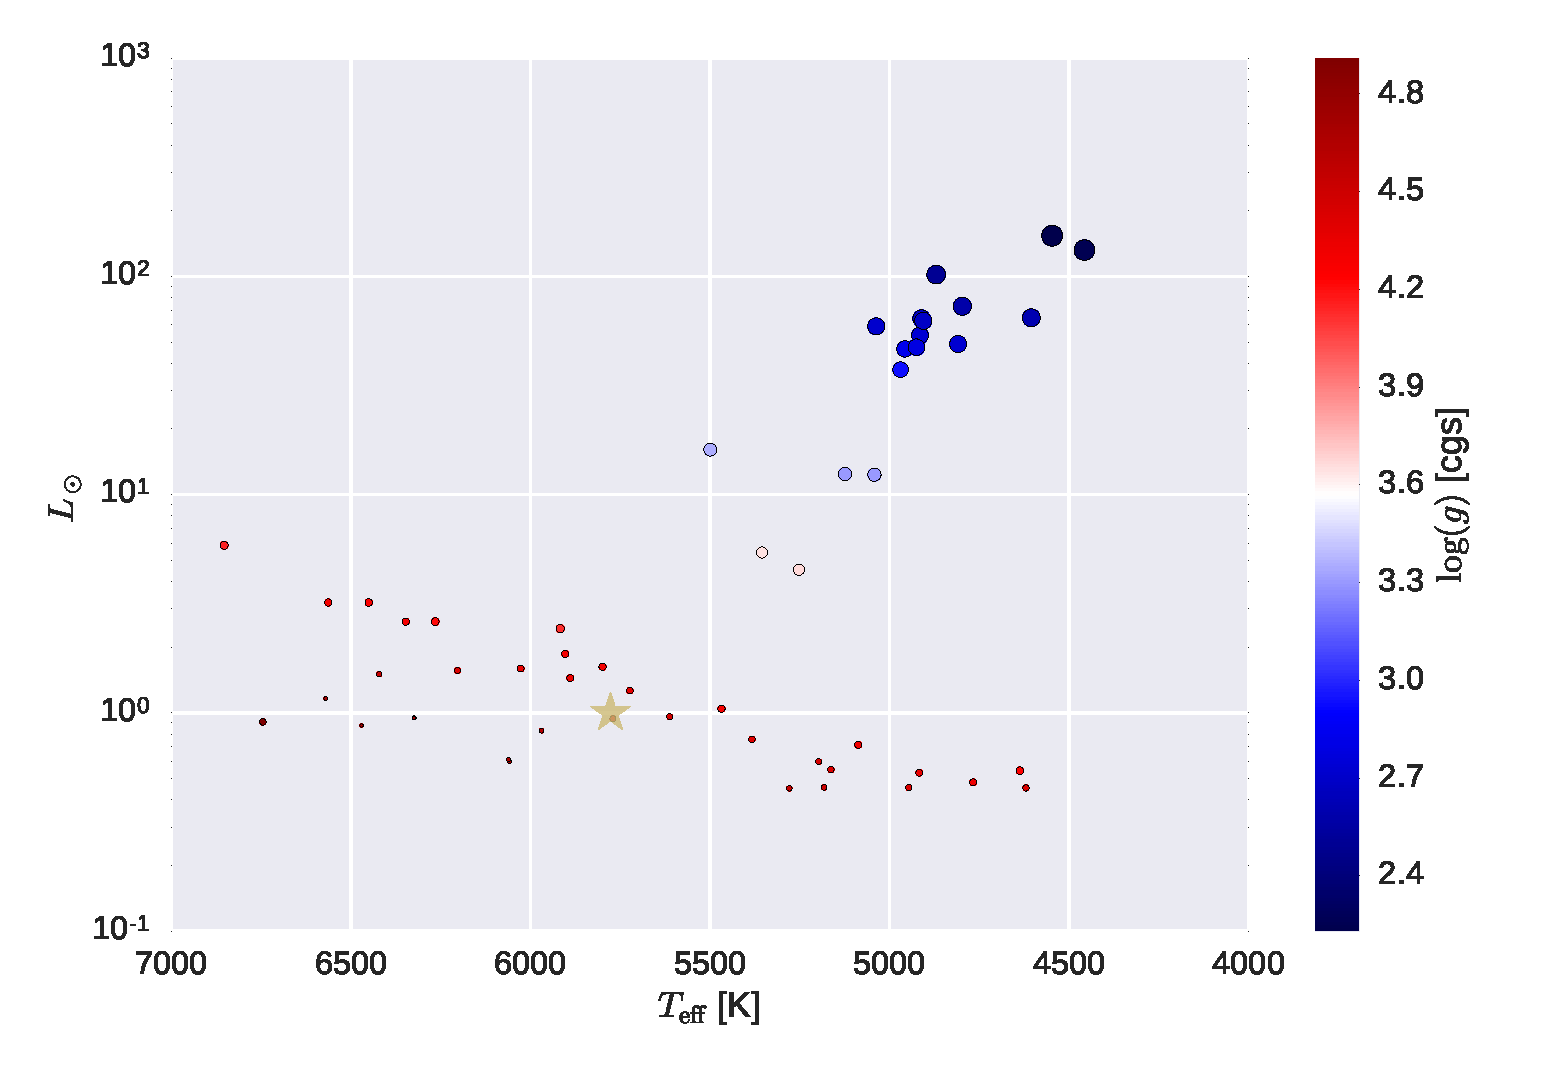
\includegraphics[width=1.0\linewidth]{figures/HR.pdf}
    \caption{Hertzprung-Russel diagram of our sample with the Sun as a yellow
    star. The size of the points represents the $\log g$, with bigger points
    being smaller $\log g$ (giants), and vice versa. The colour code show the
    same as the size. Red points are the dwarfs, while blue points are the
    giants.}
    \label{fig:HRD}
\end{figure}

\begin{figure}[tpb]
    \centering
    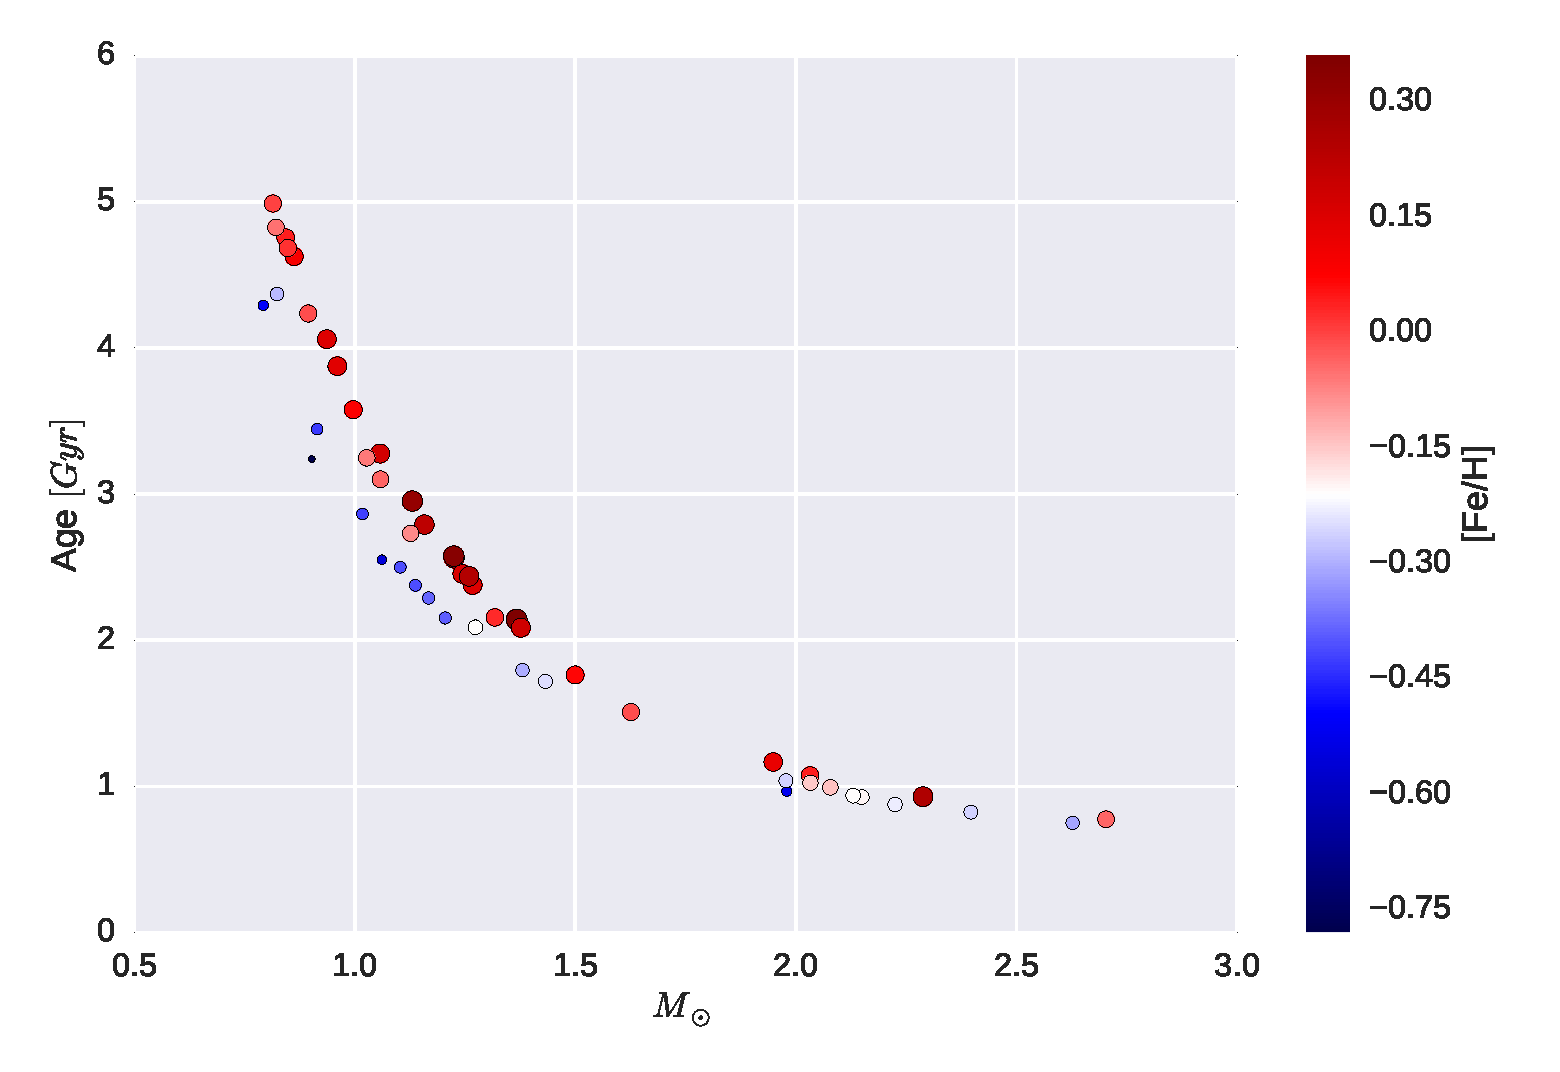
\includegraphics[width=1.0\linewidth]{figures/mass_age_feh.pdf}
    \caption{Age versus mass for our sample, with colours representing the
    [\ion{Fe}/\ion{H}].}
    \label{fig:age}
\end{figure}

We present a histogram of $T_\mathrm{eff}$ and $[\ion{Fe}/\ion{H}]$ in
% Figure~\ref{fig:update} of SWEET-Cat after this update. With 2461 stars
discovered with planets, 21\% of these stars have been analyzed in the
homogeneous way as described in this work. We note that the limiting factor at
the moment for increasing the sample of stars analyzed in the homogeneous way is
the magnitude of that planet hosts. There have been found many planet hosts with
space mission as \emph{Kepler} and \emph{CoRoT} using the transiting method.
Most of these stars are faint and thus making them time expensive for the
spectroscopic analysis required her.

% \begin{figure}[tpb]
%     \centering
%     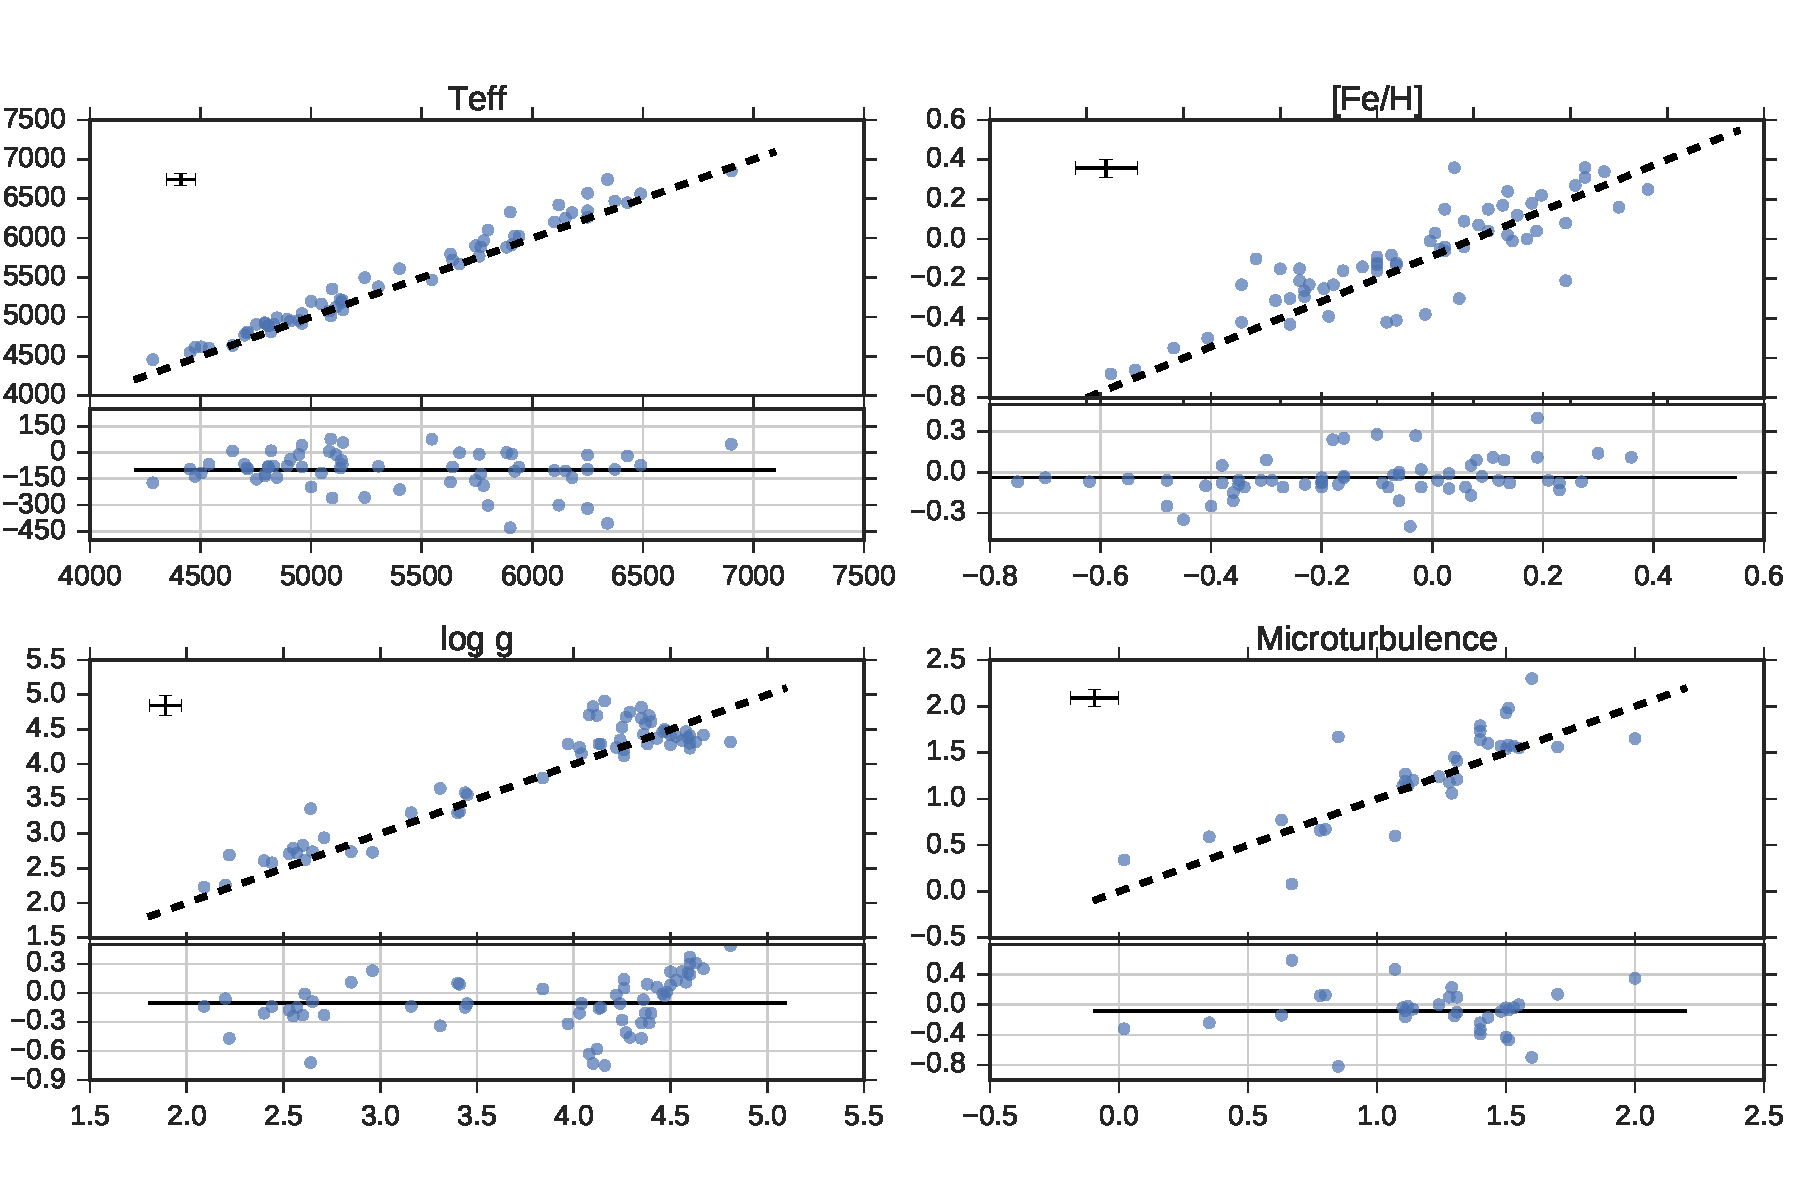
\includegraphics[width=1.0\linewidth]{figures/update.pdf}
%     \caption{Histograms of SWEET-Cat after the update.}
%     \label{fig:update}
% \end{figure}




\section{Conclusion}
\label{sec:conclusion}




\begin{acknowledgements}

This work was supported by Funda\c{c}\~ao para a Ci\^encia e a Tecnologia (FCT)
through the research grants UID/FIS/04434/2013 and PTDC/FIS-AST/1526/2014.
N.C.S., and S.G.S. acknowledge the support from FCT through Investigador FCT
contracts of reference IF/00169/2012, and IF/00028/2014, respectively, and
POPH/FSE (EC) by FEDER funding through the program “Programa Operacional de
Factores de Competitividade - COMPETE”. E.D.M. and B.J.A. acknowledge the
support from FCT in form of the fellowship SFRH/BPD/76606/2011 and
SFRH/BPD/87776/2012, respectively. This work also benefit from the collaboration
of a cooperation project FCT/CAPES - 2014/2015 (FCT Proc 4.4.1.00 CAPES).

AM received funding from the European Union Seventh Framework Programme
(FP7/2007-2013) under grant agreement number 313014 (ETAEARTH).

This research has made use of the SIMBAD database operated at CDS, Strasbourg
(France).

\end{acknowledgements}


\bibpunct{(}{)}{;}{a}{}{,}
\bibliographystyle{aa}
\bibliography{thesis}



\end{document}
